\documentclass[border=4pt]{standalone}
\usepackage{tikz}
\usepackage{pgfplots}
\pgfplotsset{compat=1.18}
\usetikzlibrary{shapes.geometric,arrows.meta,positioning,calc,fit,decorations.pathreplacing,backgrounds}
\definecolor{boxblue}{RGB}{225,238,252}
\definecolor{boxgreen}{RGB}{225,247,231}
\definecolor{boxorange}{RGB}{253,236,216}
\definecolor{boxgray}{RGB}{237,237,237}
\definecolor{boxred}{RGB}{253,226,226}
\begin{document}
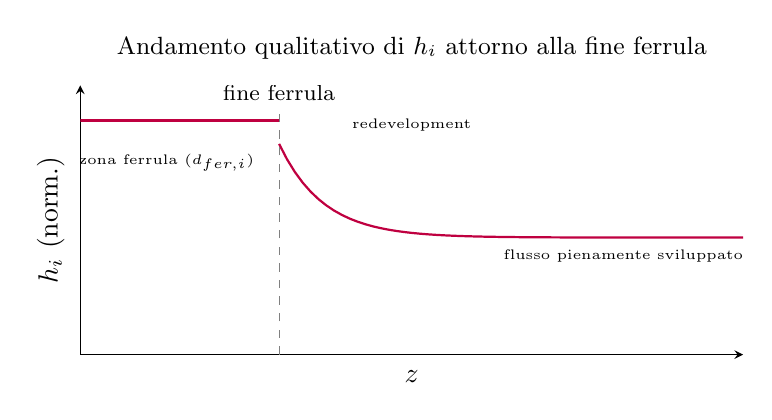
\begin{tikzpicture}
\begin{axis}[
  width=10cm, height=5cm,
  xlabel={$z$}, ylabel={$h_i$ (norm.)},
  xtick=\empty, ytick=\empty,
  axis lines=left,
  ymin=0, ymax=1.15, xmin=0, xmax=1,
  title={\small Andamento qualitativo di $h_i$ attorno alla fine ferrula},
]
\addplot[thick,purple,domain=0:0.3,samples=2]{1.0};
\addplot[thick,purple,domain=0.3:1,samples=60]{0.5+0.4*exp(-15*(x-0.3))};
\draw[dashed,gray] (axis cs:0.3,0) -- (axis cs:0.3,1.05);
\node[font=\footnotesize] at (axis cs:0.3,1.12) {fine ferrula};
\node[font=\tiny] at (axis cs:0.13,0.82) {zona ferrula ($d_{fer,i}$)};
\node[font=\tiny] at (axis cs:0.5,0.98) {redevelopment};
\node[font=\tiny] at (axis cs:0.85,0.42) {flusso pienamente sviluppato ($d_i$)};
\end{axis}
\end{tikzpicture}
\end{document}
